\section{Sub\-Bar\-Close Class Reference}
\label{classSubBarClose}\index{SubBarClose@{SubBarClose}}
{\tt \#include $<$subbarclose.h$>$}

Inheritance diagram for Sub\-Bar\-Close:\begin{figure}[H]
\begin{center}
\leavevmode
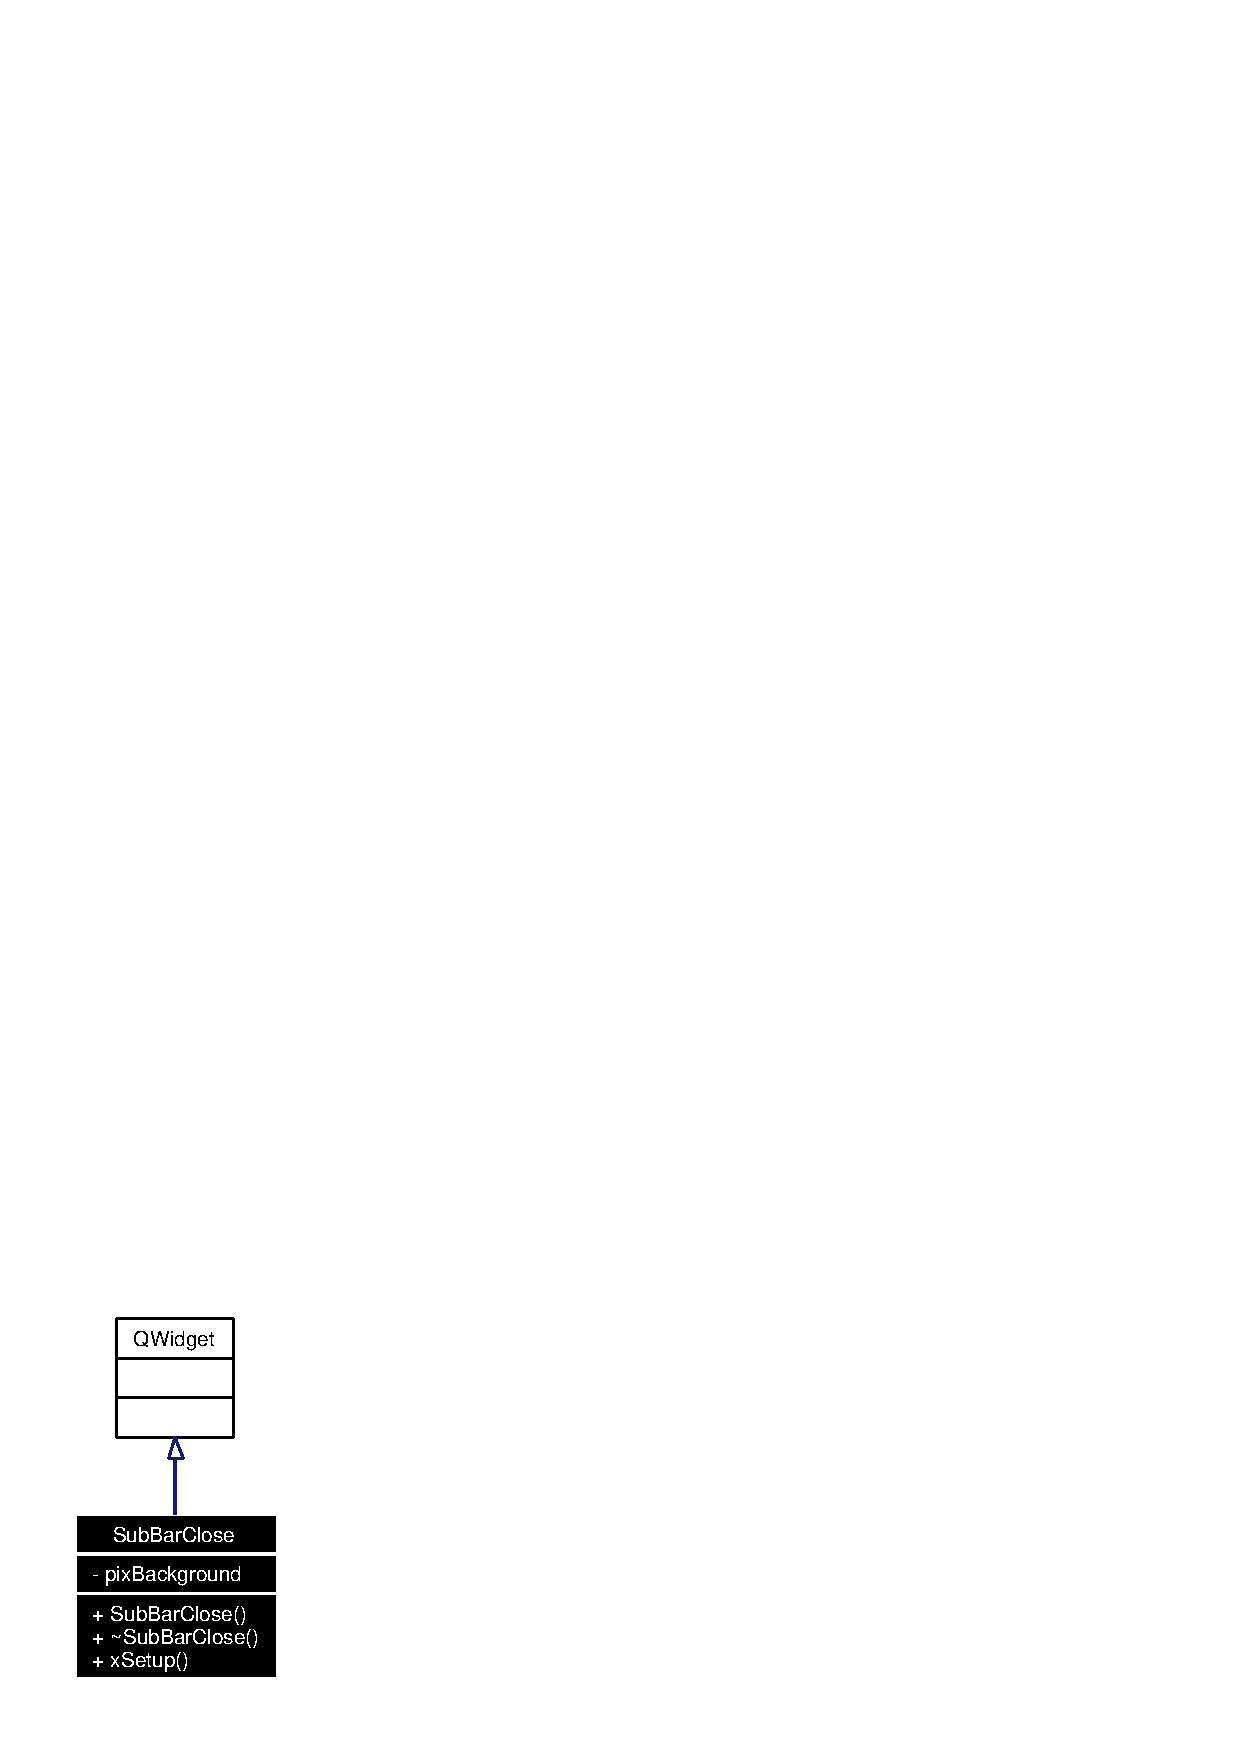
\includegraphics[width=66pt]{classSubBarClose__inherit__graph}
\end{center}
\end{figure}
Collaboration diagram for Sub\-Bar\-Close:\begin{figure}[H]
\begin{center}
\leavevmode
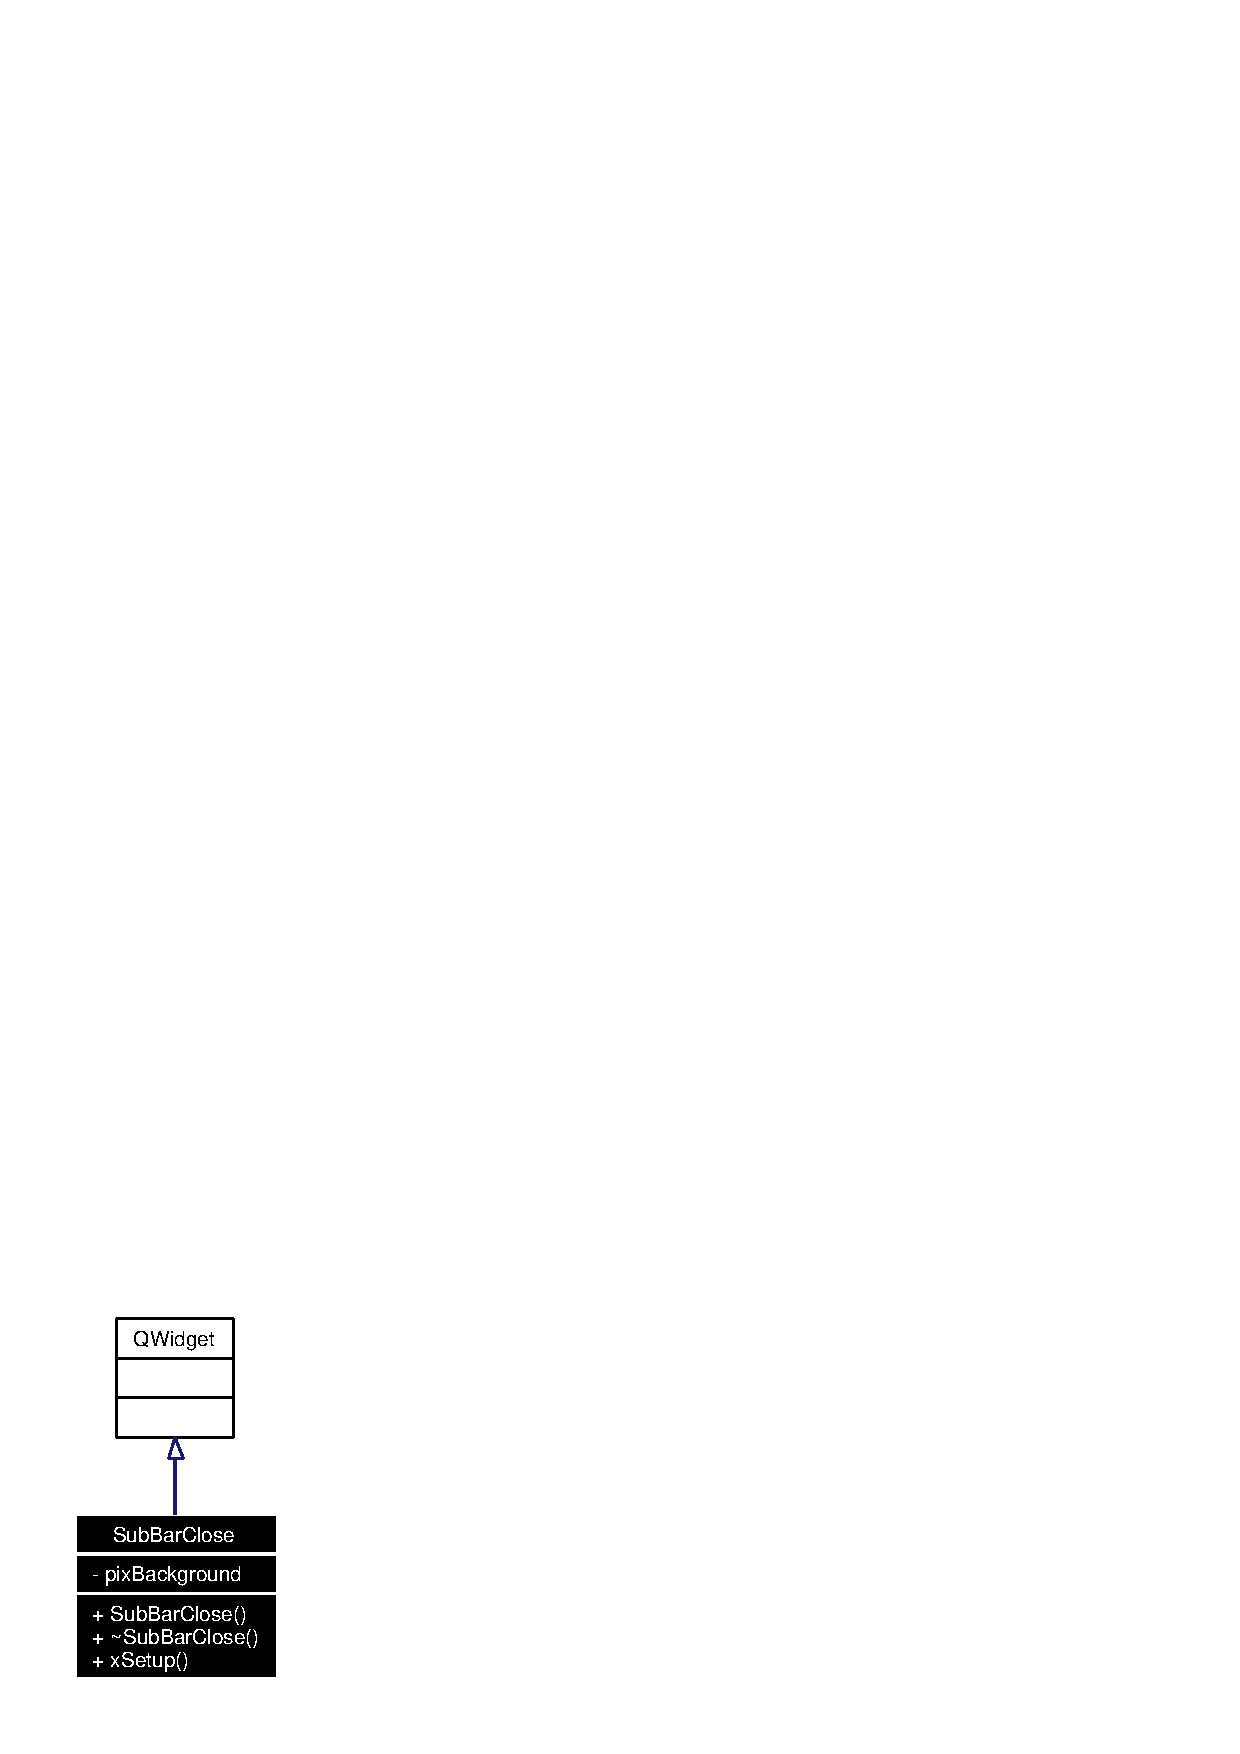
\includegraphics[width=66pt]{classSubBarClose__coll__graph}
\end{center}
\end{figure}


\subsection{Detailed Description}
\begin{Desc}
\item[Author:]sonicat \end{Desc}




Definition at line 28 of file subbarclose.h.\subsection*{Public Member Functions}
\begin{CompactItemize}
\item 
{\bf Sub\-Bar\-Close} ({\bf QWidget} $\ast$parent=0, const char $\ast$name=0)
\item 
{\bf $\sim$Sub\-Bar\-Close} ()
\item 
void {\bf x\-Setup} ()
\end{CompactItemize}
\subsection*{Private Attributes}
\begin{CompactItemize}
\item 
QPixmap {\bf pix\-Background}
\end{CompactItemize}


\subsection{Constructor \& Destructor Documentation}
\index{SubBarClose@{Sub\-Bar\-Close}!SubBarClose@{SubBarClose}}
\index{SubBarClose@{SubBarClose}!SubBarClose@{Sub\-Bar\-Close}}
\subsubsection{\setlength{\rightskip}{0pt plus 5cm}Sub\-Bar\-Close::Sub\-Bar\-Close ({\bf QWidget} $\ast$ {\em parent} = 0, const char $\ast$ {\em name} = 0)}\label{classSubBarClose_SubBarClosea0}




Definition at line 22 of file subbarclose.cpp.

References x\-Setup().



\footnotesize\begin{verbatim}23  : QWidget(parent, name)
24 {
25   xSetup();
26 }
\end{verbatim}\normalsize 


Here is the call graph for this function:\begin{figure}[H]
\begin{center}
\leavevmode
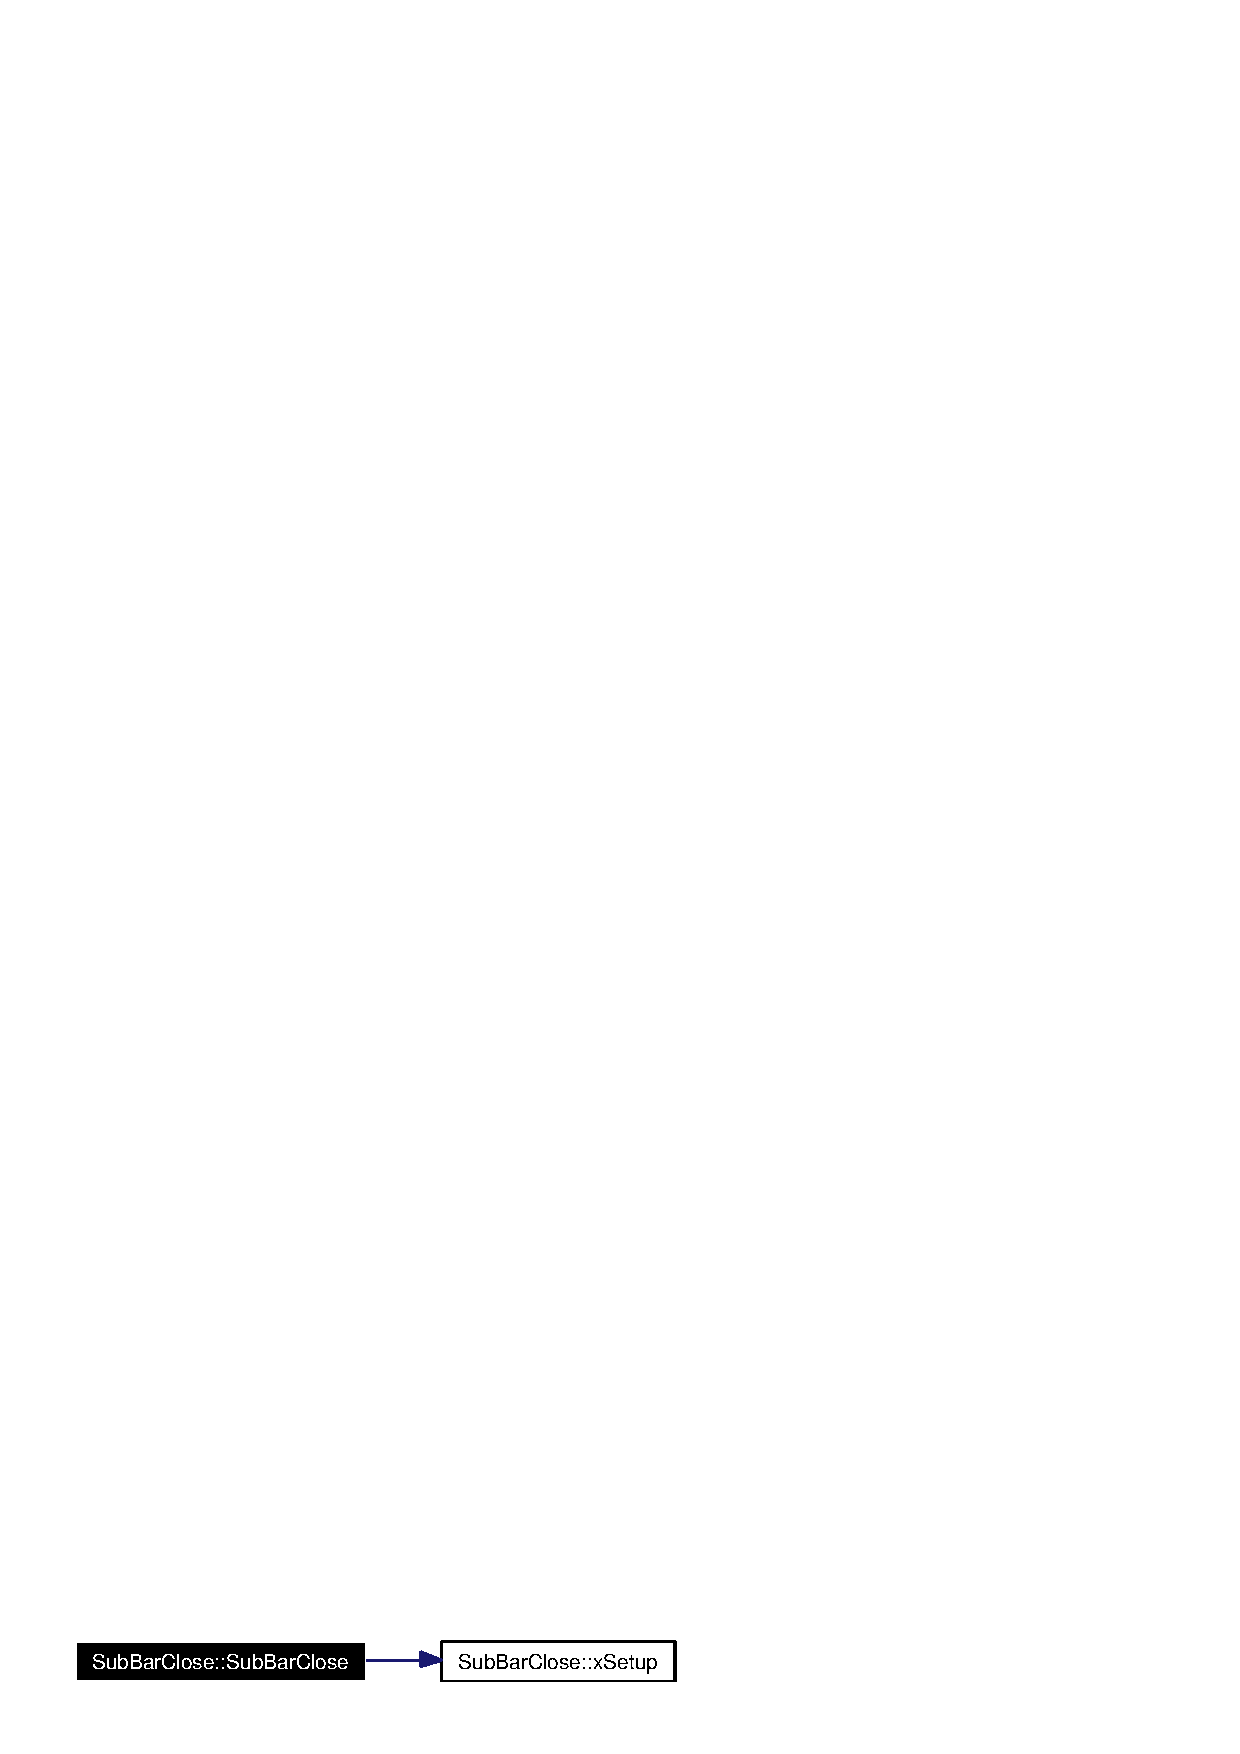
\includegraphics[width=162pt]{classSubBarClose_SubBarClosea0_cgraph}
\end{center}
\end{figure}
\index{SubBarClose@{Sub\-Bar\-Close}!~SubBarClose@{$\sim$SubBarClose}}
\index{~SubBarClose@{$\sim$SubBarClose}!SubBarClose@{Sub\-Bar\-Close}}
\subsubsection{\setlength{\rightskip}{0pt plus 5cm}Sub\-Bar\-Close::$\sim${\bf Sub\-Bar\-Close} ()}\label{classSubBarClose_SubBarClosea1}




Definition at line 29 of file subbarclose.cpp.



\footnotesize\begin{verbatim}30 {
31 }
\end{verbatim}\normalsize 


\subsection{Member Function Documentation}
\index{SubBarClose@{Sub\-Bar\-Close}!xSetup@{xSetup}}
\index{xSetup@{xSetup}!SubBarClose@{Sub\-Bar\-Close}}
\subsubsection{\setlength{\rightskip}{0pt plus 5cm}void Sub\-Bar\-Close::x\-Setup ()}\label{classSubBarClose_SubBarClosea2}




Definition at line 32 of file subbarclose.cpp.

Referenced by Sub\-Bar\-Close().



\footnotesize\begin{verbatim}33 {
34    //DAVID Setup Background;
35    pixBackground.load("/root/kde_application/hdass08/skin/SubBarBackground.png");
36    setBackgroundPixmap(pixBackground);
37 }
\end{verbatim}\normalsize 


\subsection{Member Data Documentation}
\index{SubBarClose@{Sub\-Bar\-Close}!pixBackground@{pixBackground}}
\index{pixBackground@{pixBackground}!SubBarClose@{Sub\-Bar\-Close}}
\subsubsection{\setlength{\rightskip}{0pt plus 5cm}QPixmap {\bf Sub\-Bar\-Close::pix\-Background}\hspace{0.3cm}{\tt  [private]}}\label{classSubBarClose_SubBarCloser0}




Definition at line 37 of file subbarclose.h.

The documentation for this class was generated from the following files:\begin{CompactItemize}
\item 
{\bf subbarclose.h}\item 
{\bf subbarclose.cpp}\end{CompactItemize}
